%!TEX program = xelatex

% \documentclass[10pt]{article}
%%%%%%%%%%%%%%%%%%%%%%%%%%%%%%%%%%%%%%%%%
% Modified By Orcuslc, 2016-9-21
% Modified for Assignments
% http://github.com/orcuslc
%
% Wilson Resume/CV
% Structure Specification File
% Version 1.0 (22/1/2015)
%
% This file has been downloaded from:
% http://www.LaTeXTemplates.com
%
% License:
% CC BY-NC-SA 3.0 (http://creativecommons.org/licenses/by-nc-sa/3.0/)
%
%%%%%%%%%%%%%%%%%%%%%%%%%%%%%%%%%%%%%%%%%

%----------------------------------------------------------------------------------------
%	PACKAGES AND OTHER DOCUMENT CONFIGURATIONS
%----------------------------------------------------------------------------------------
\documentclass[10pt]{article}

\usepackage{listings}
\usepackage{xcolor}
\usepackage{amsmath,amsthm,amssymb}
\usepackage{epstopdf}
\usepackage{graphicx}
\usepackage{clrscode3e}

\DeclareGraphicsExtensions{.eps,.ps,.jpg,.bmp}


\usepackage[a4paper, hmargin=25mm, vmargin=30mm, top=20mm]{geometry} % Use A4 paper and set margins

\usepackage{fancyhdr} % Customize the header and footer

\usepackage{lastpage} % Required for calculating the number of pages in the document

\usepackage{hyperref} % Colors for links, text and headings

\setcounter{secnumdepth}{0} % Suppress section numbering

%\usepackage[proportional,scaled=1.064]{erewhon} % Use the Erewhon font
%\usepackage[erewhon,vvarbb,bigdelims]{newtxmath} % Use the Erewhon font
\usepackage[utf8]{inputenc} % Required for inputting international characters
\usepackage[T1]{fontenc} % Output font encoding for international characters

\usepackage{fontspec} % Required for specification of custom fonts
\setmainfont[Path = ./fonts/,
Extension = .otf,
BoldFont = Erewhon-Bold,
ItalicFont = Erewhon-Italic,
BoldItalicFont = Erewhon-BoldItalic,
SmallCapsFeatures = {Letters = SmallCaps}
]{Erewhon-Regular}

\usepackage{color} % Required for custom colors
\definecolor{slateblue}{rgb}{0.17,0.22,0.34}

\usepackage{sectsty} % Allows customization of titles
\sectionfont{\color{slateblue}} % Color section titles

\fancypagestyle{plain}{\fancyhf{}\cfoot{\thepage\ of \pageref{LastPage}}} % Define a custom page style
\pagestyle{plain} % Use the custom page style through the document
\renewcommand{\headrulewidth}{0pt} % Disable the default header rule
\renewcommand{\footrulewidth}{0pt} % Disable the default footer rule

\setlength\parindent{0pt} % Stop paragraph indentation

% Non-indenting itemize
\newenvironment{itemize-noindent}
{\setlength{\leftmargini}{0em}\begin{itemize}}
{\end{itemize}}

% Text width for tabbing environments
\newlength{\smallertextwidth}
\setlength{\smallertextwidth}{\textwidth}
\addtolength{\smallertextwidth}{-2cm}

\newcommand{\sqbullet}{~\vrule height .8ex width .6ex depth -.05ex} % Custom square bullet point 


\newcommand{\tbf}[1]{\textbf{#1}}
\newcommand{\tit}[1]{\textit{#1}}
\newcommand{\mbb}[1]{\mathbb{#1}}
\newcommand{\blue}[1]{\color{blue}{#1}}
\newcommand{\red}[1]{\color{red}{#1}}
\newcommand{\sblue}[1]{\color{slateblue}{#1}}
\newcommand{\n}{\\[5pt]}
\newcommand{\tr}{^\top}
\newcommand{\vt}[1]{
\Vert #1 \Vert
}
\newcommand{\bra}[5]{
#1=\left\{
\begin{aligned}
#2 ,&\quad #4 \\
#3 ,&\quad #5
\end{aligned}
\right.
}

\renewcommand{\title}[2] {
{\Huge{\color{slateblue}\textbf{#1}}}
\hfill
\LARGE{\color{slateblue}\textbf{#2}} \\[10pt]
\large{\color{slateblue}\textbf{Chuan Lu, 13300180056, chuanlu13@fudan.edu.cn}} \\[1mm]
\rule{\textwidth}{0.5mm}
}

\newcommand{\problem}[2] {
\vspace{20pt}
\LARGE{\color{slateblue}\textbf{Problem #1.}}
\vspace{2mm}
#2 \\[10pt]
}

\renewcommand{\proof}[2] {
\large{\color{slateblue}\textit{\textbf{#1.}}}
#2 \qed \\[3mm]
}

\newcommand{\solution}[2] {
\large{\color{slateblue}\textit{\textbf{#1.}}}
#2 \\[3mm]
}


\newcommand{\algorithm}[2] {
\begin{codebox}
\Procname{$\proc{Algorithm #1}$}
#2
\end{codebox}
}

\newcommand{\refgroup}[1] {
\LARGE{\color{slateblue}\textbf{Reference}} 
\begin{tabbing}
\hspace{5mm} \= \kill
#1
\end{tabbing}
}

\newcommand{\reference}[1] {
\sqbullet \ \  \large{#1} \\
}
% \newcommand{\solution}[2] {
% \LARGE{\color{slateblue}\textit{#1}}
% \ #2 \qed
% }

% \newenvironment{problem}[2][Problem]{\begin{trivlist}
% \item[\hskip \labelsep {\bfseries #1}\hskip \labelsep {\bfseries #2.}]}{\end{trivlist}}
\usepackage{epstopdf}
\usepackage{graphics}
\usepackage{subfig}
\usepackage{listings}
\lstset{
  numbers=left,
    framexleftmargin=10mm,
    frame=none,
    backgroundcolor=\color[RGB]{245,245,244},
  keywordstyle=\bf\color{blue},
  identifierstyle=\bf,
  numberstyle=\color[RGB]{0,192,192},
  commentstyle=\it\color[RGB]{0,96,96},
  stringstyle=\rmfamily\slshape\color[RGB]{128,0,0},
  showstringspaces=false,
  extendedchars=false
    }
\DeclareGraphicsExtensions{.eps,.ps,.jpg,.bmp}

\begin{document}

\title{Homework 2}{16.10.9}

% \parbox{0.3\textwidth}{
% Chuan Lu}
% \hfill
% \parbox{0.3\textwidth}{
% 13300180056}
% \hfill
% \parbox{0.3\textwidth}{
% chuanlu13@fudan.edu.cn}

\problem{1}{Explain the relationship between spectral clustering, normalized spectral clustering and graph cut.}
\solution{Solution}{
We assume $k=2$ in the following explanation. \n
For spectral clustering, we already know that the eigenvector $u_2$ corresponding to the second smallest eigenvalue $\lambda_2$ of the Laplacian matrix of the graph is the solution for the minimization
$$ \min_{\tbf{f}} \ \tbf{f}^\top\tbf{L}\tbf{f},$$
$$s.t. \quad \tbf{f}^\top \tbf{f} = 1, \tbf{f}^\top\tbf{1} = 0$$
In fact, if we define 
$$G(f) = G(f_1,\cdots, f_n) = f\tr\tbf{L}f - \lambda_1 (f\tr f-1) - \lambda_2 f\tr\tbf{1} $$ $$ =  \frac{1}{2}\sum_{i,j=1}^{n}w_{ij}(f_i-f_j)^2-\lambda_1(\sum_{i=1}^{n}f_i^2-1)-\lambda_2\sum_{i=1}^n f_i$$
Then according to Lagrange Theorm, we let
$$\frac{\partial G}{\partial f_i} = \sum_{j=1}^n (f_i-f_j) - 2\lambda_1 f_i - \lambda_2 = 0, \quad  i=1:n$$
If we add the $n$ equations, we get
$$2\lambda_1\sum_{i, j=1}^n f_i + n\lambda_2=0$$
Since $f\tr\tbf{1} = 0$, then $\lambda_2 = 0$. So
$$\sum_{j=1}^n w_{ij}f_{j} = \lambda f_i, \quad i=1:n,$$
which means $f$ is an eigenvector of $\tbf{L}$.\n
For Min Cut, if we define $\tbf{f} = (f_1, f_2\cdots f_n)^\top$
}

% \problem{2}{Cluster $Data_i.csv$ with K-means, judge the number of clusters, and compare differences between different evaluating methods.}
% \solution{Solution}{
% The code of K-means, evaluating and test scripts can be found from attachments(kmeans.R, evaluate.R, hw1.2.R).
% }
% \solution{Result}{
% For Data1.csv, we cluster with k = 3. The result is shown as below.
% \begin{figure}[htbp]
% \centering
% 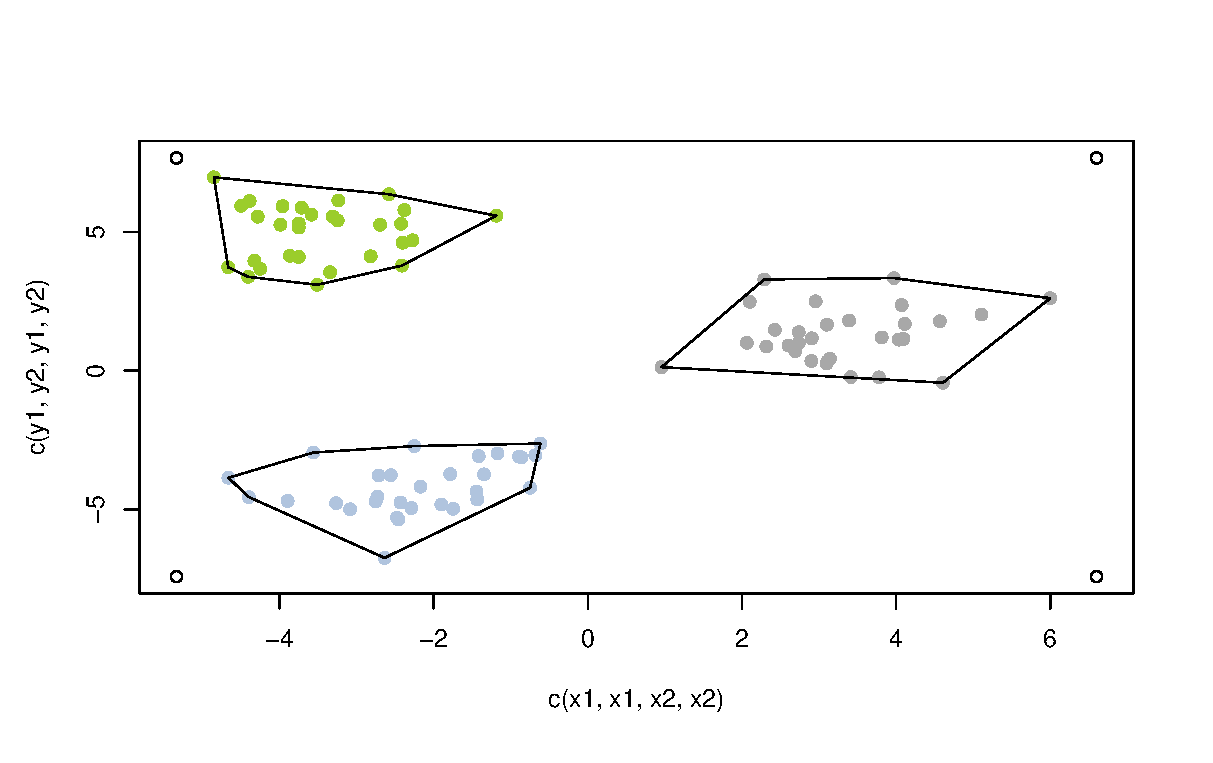
\includegraphics[width = 15cm]{pics/hw2_data1_cluster.eps}
% \caption{The clusters of Data1.csv with k = 3}
% \label{clusters of data1}
% \end{figure}
% \\[1mm]

% For choosing k, the result of Data1.csv is shown below; The first is the result of Calinski-Harabasz method, the second Hartigan method and the last Gap Statistic. \\[3pt]
% The result of CH method is 9, if we may add a limit that $k\le 10.$ The result of H method is 3, and result of GAP statistic is 3.\\[3pt]

% \begin{figure}[htbp]
% \centering
% \subfloat[CH method]{ %
% 	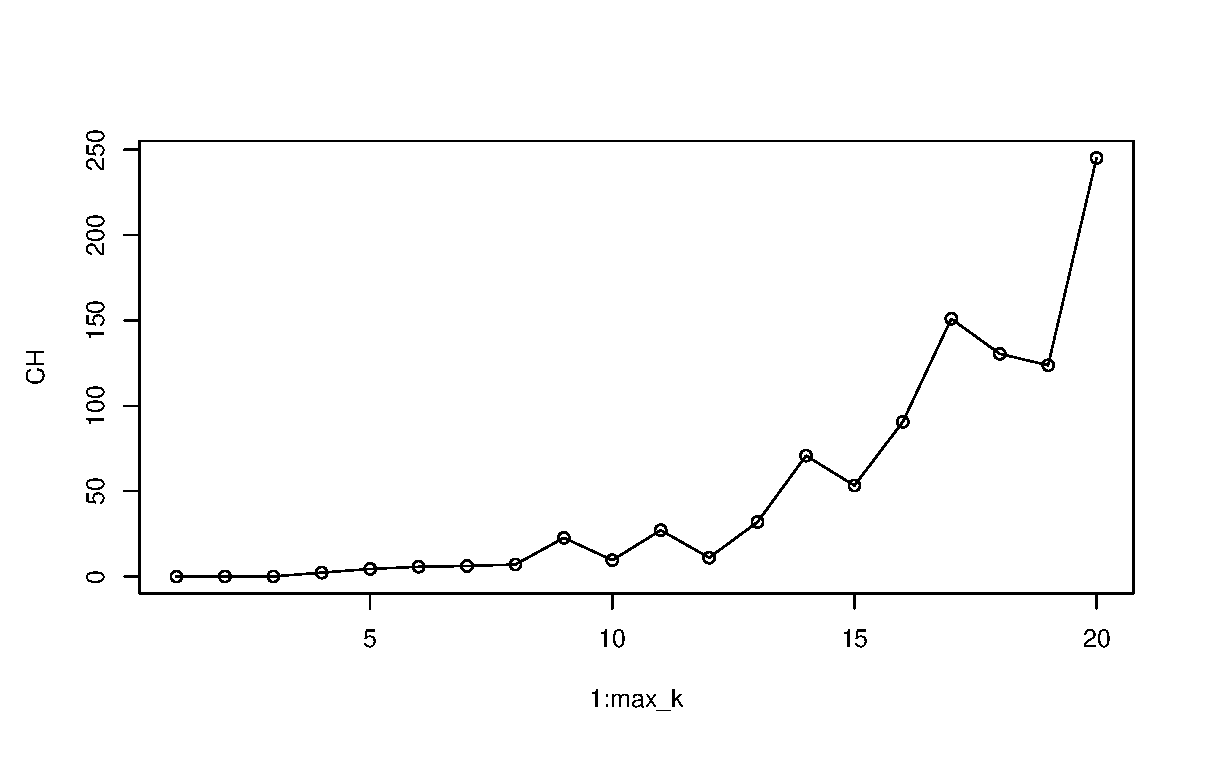
\includegraphics[width = 0.3\textwidth]{pics/hw2_data1_k_CH.eps}}\hfill
% \subfloat[H method]{ %
% 	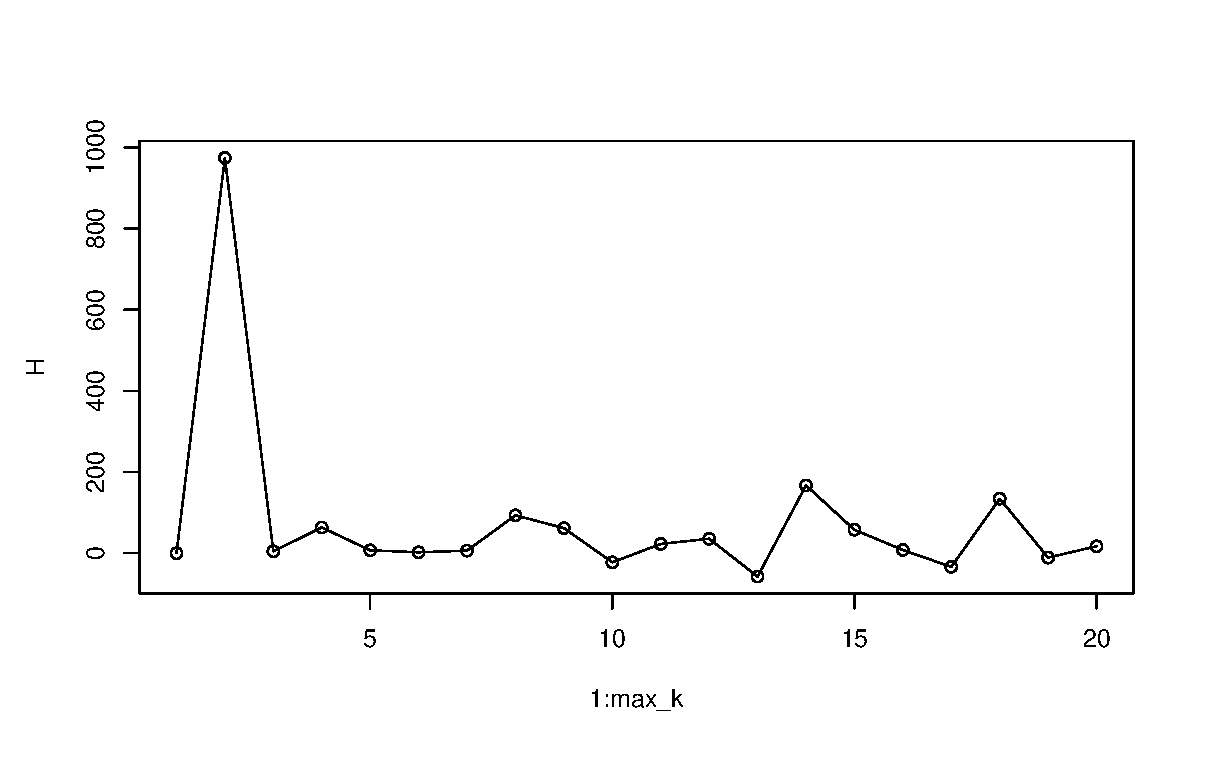
\includegraphics[width = 0.3\textwidth]{pics/hw2_data1_k_H.eps}}\hfill
% \subfloat[GAP statistic]{ %
% 	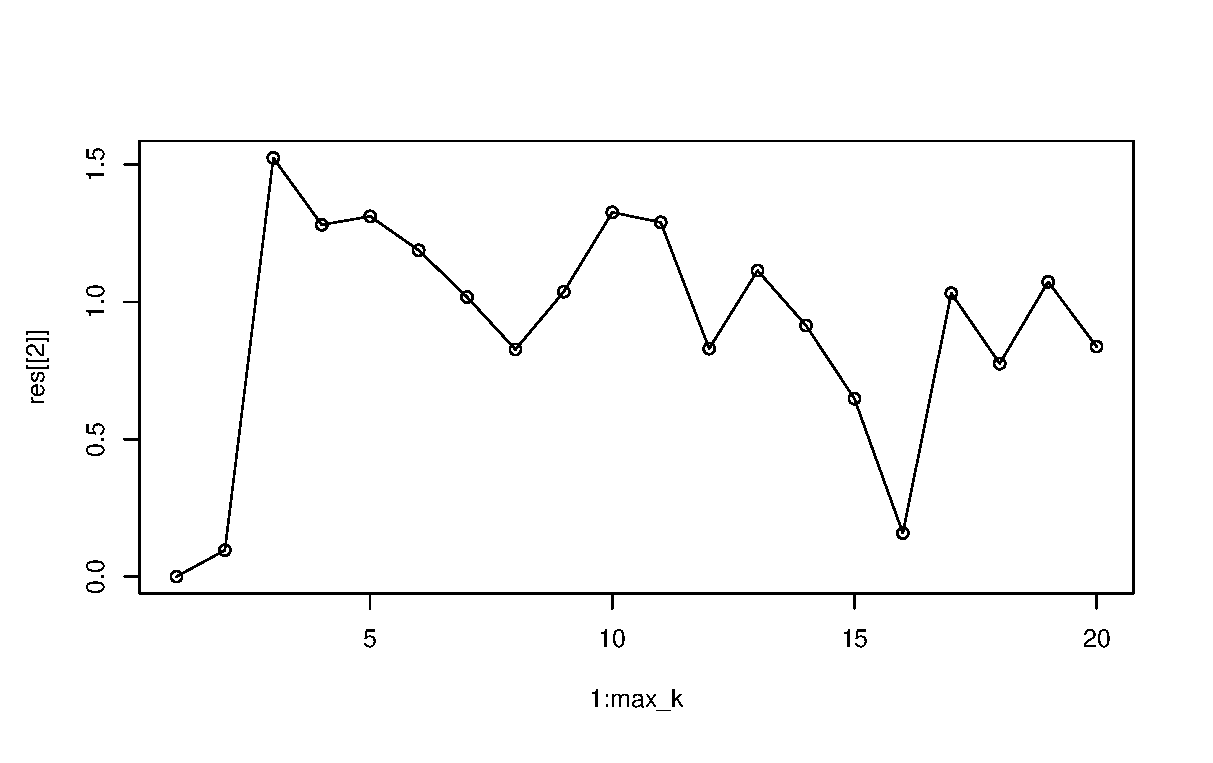
\includegraphics[width = 0.3\textwidth]{pics/hw2_data1_k_GAP.eps}}\hfill
% \caption{The three evaluating methods of choosing k for Data1.csv}
% \label{EVA Data1}
% \end{figure}

% For Data2.csv, since each data point is of 3 dims, we cannot plot its clustering result here. But after deploying the evaluating methods we consider k = 3. The type of datas can be find in attachments(CLUSTER\_DATA2.txt). \\[3pt]

% The result of CH method is 8, if we limit that $k\le 10$. The result of H method and result of GAP statistic are 3. \\[3pt]
% The pics are shown below.

% \begin{figure}[htbp]
% \centering
% \subfloat[CH method]{ %
% 	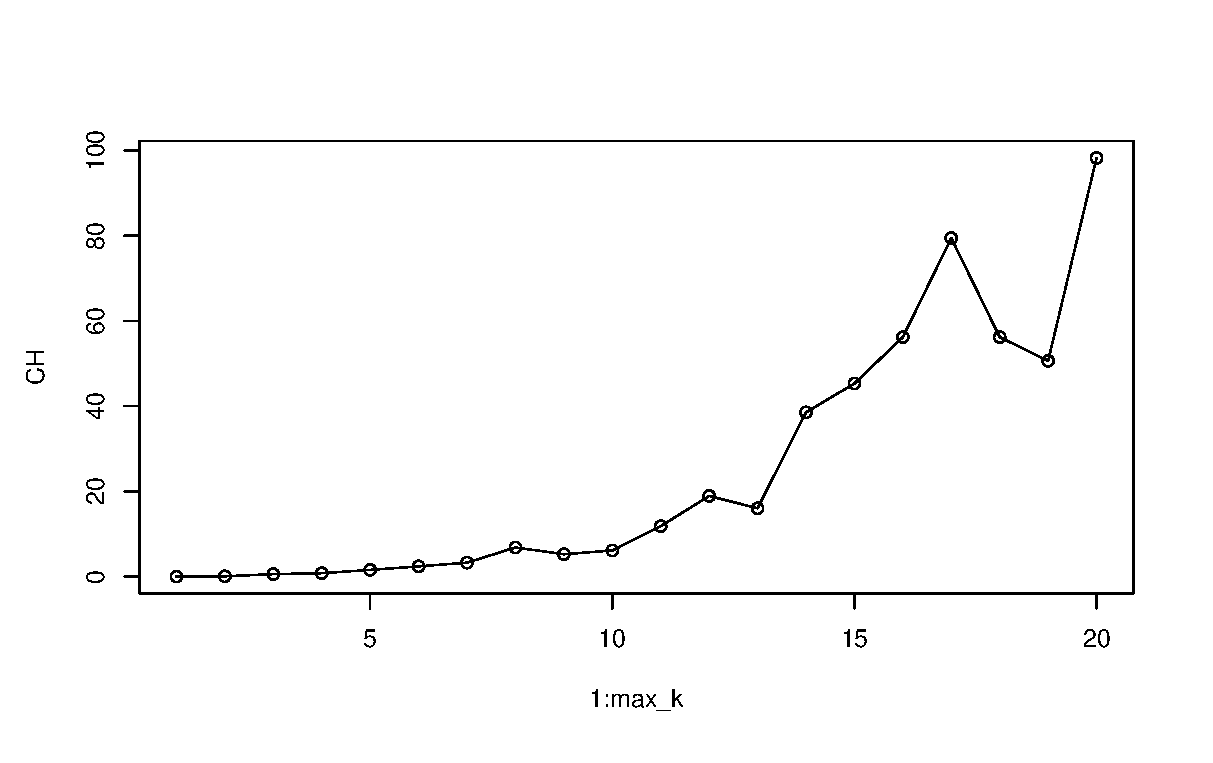
\includegraphics[width = 0.3\textwidth]{pics/hw2_data2_k_CH.eps}}\hfill
% \subfloat[H method]{ %
% 	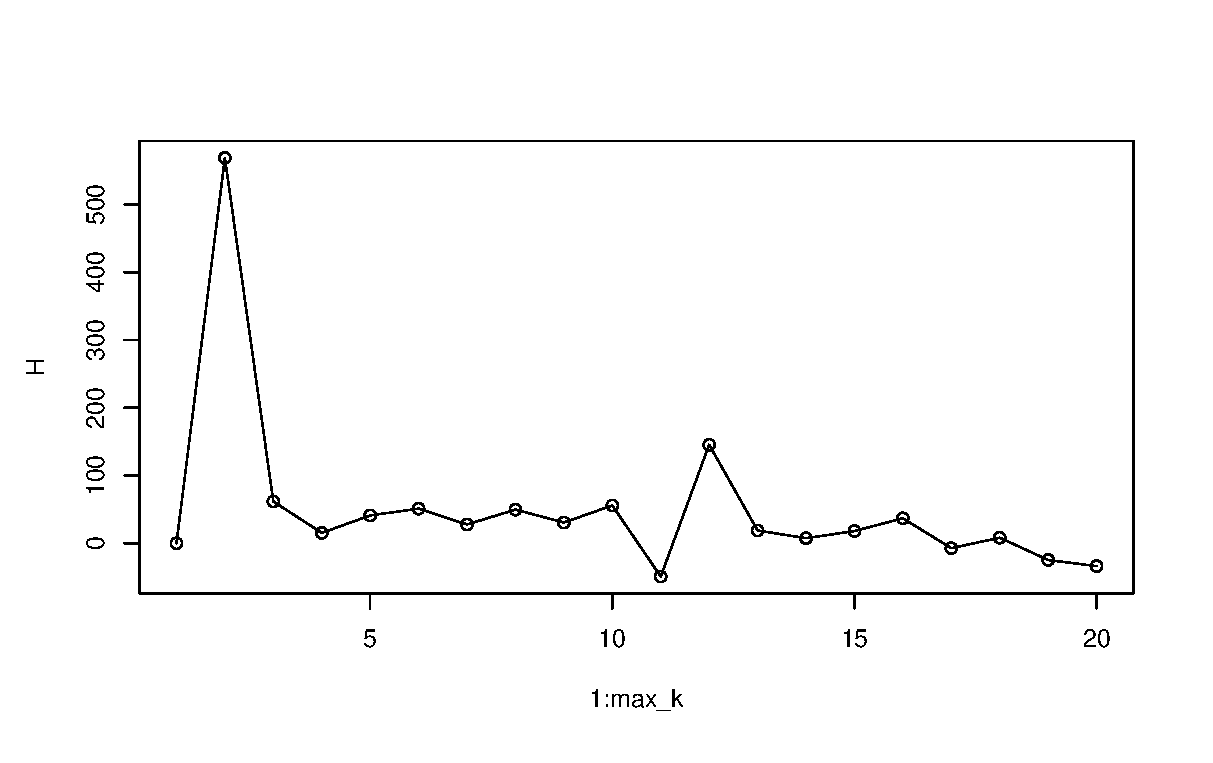
\includegraphics[width = 0.3\textwidth]{pics/hw2_data2_k_H.eps}}\hfill
% \subfloat[GAP statistic]{ %
% 	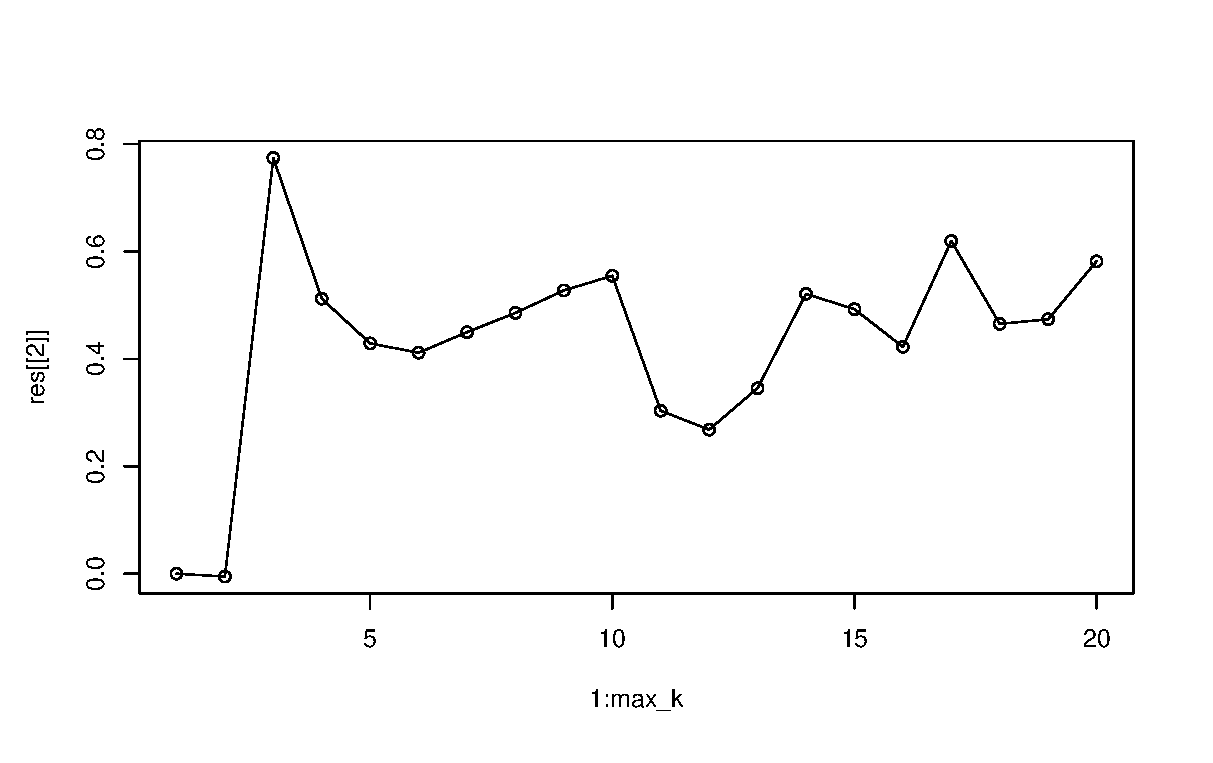
\includegraphics[width = 0.3\textwidth]{pics/hw2_data2_k_GAP.eps}}\hfill
% \caption{The three evaluating methods of choosing k for Data2.csv}
% \label{EVA Data2}
% \end{figure}

% For Data3.csv, we fix k = 3 after evaluating k with H method and GAP statistic; The result of clustering can be found in attachments(CLUSTER\_DATA3.txt). \\[3pt]

% The result of CH method is 9, if we limit that $k\le 10$. The result of H method and result of GAP statistic are 3. \\[3pt]
% The pics are shown below.

% \begin{figure}[htbp]
% \centering
% \subfloat[CH method]{ %
% 	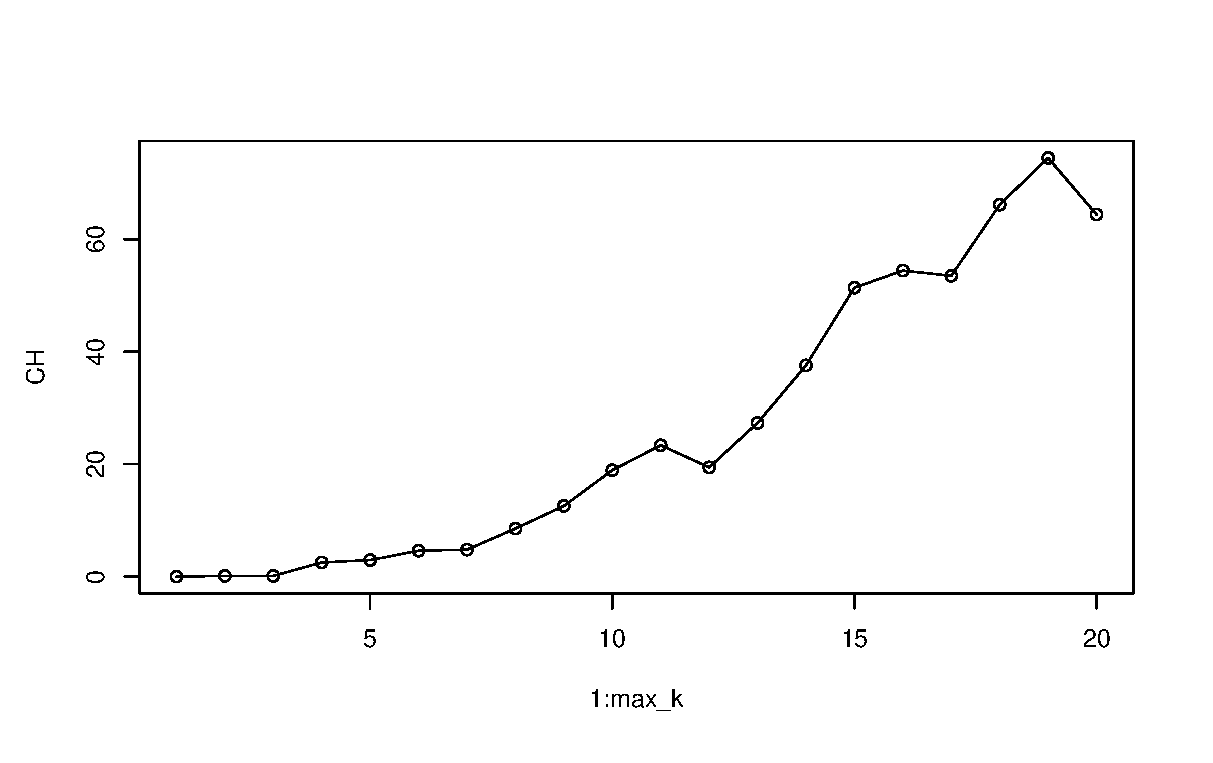
\includegraphics[width = 0.3\textwidth]{pics/hw2_data3_k_CH.eps}}\hfill
% \subfloat[H method]{ %
% 	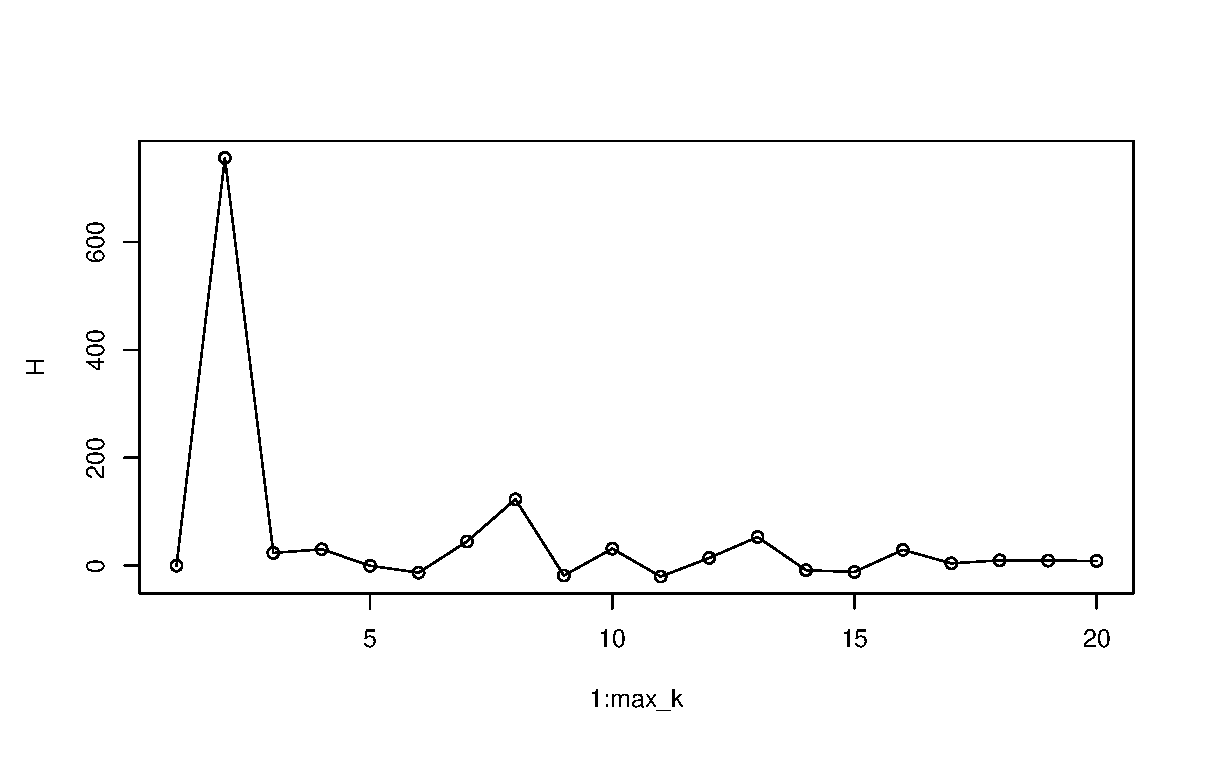
\includegraphics[width = 0.3\textwidth]{pics/hw2_data3_k_H.eps}}\hfill
% \subfloat[GAP statistic]{ %
% 	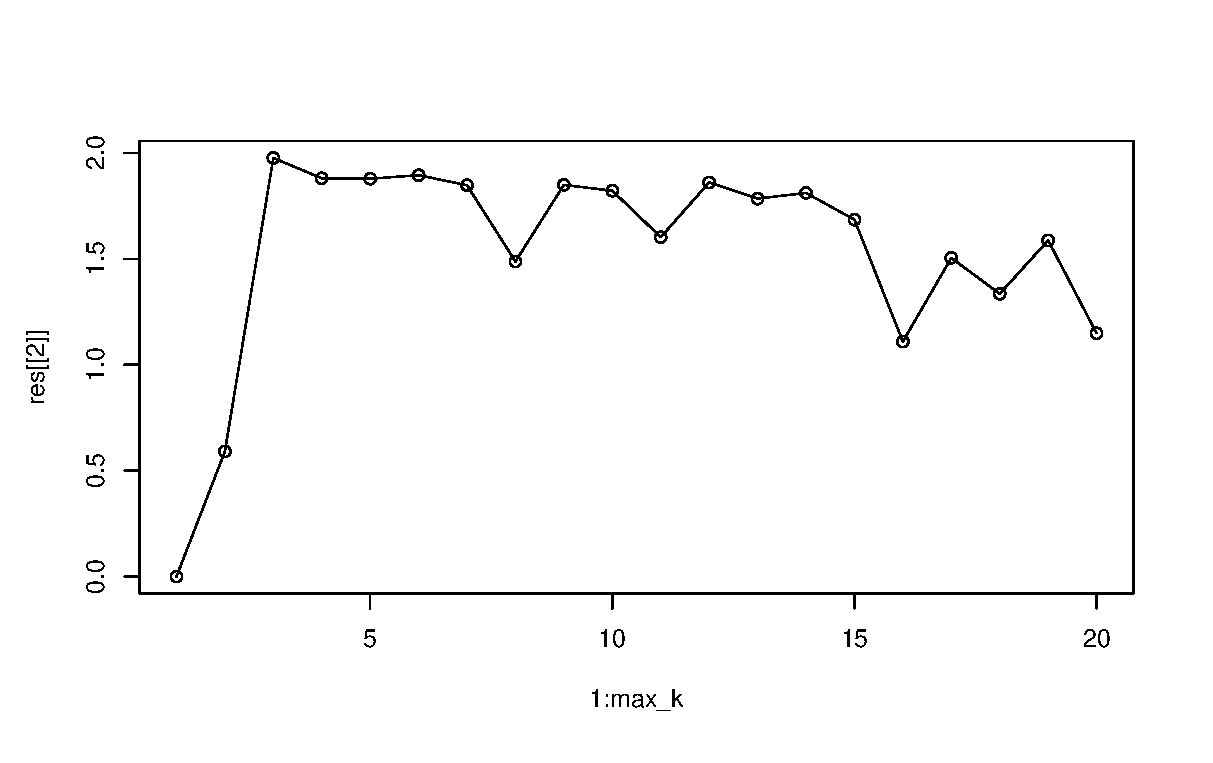
\includegraphics[width = 0.3\textwidth]{pics/hw2_data3_k_GAP.eps}}\hfill
% \caption{The three evaluating methods of choosing k for Data3.csv}
% \label{EVA Data2}
% \end{figure}

% For Data4.csv, we found k = 3 after evaluating k with H method and GAP statistic; The result of clustering can be found in attachments(CLUSTER\_DATA4.txt). \\[3pt]

% The result of CH method is 7, if we limit that $k\le 10$. The result of H method and result of GAP statistic are 3. \\[3pt]
% The pics are shown below.

% \begin{figure}[htbp]
% \centering
% \subfloat[CH method]{ %
% 	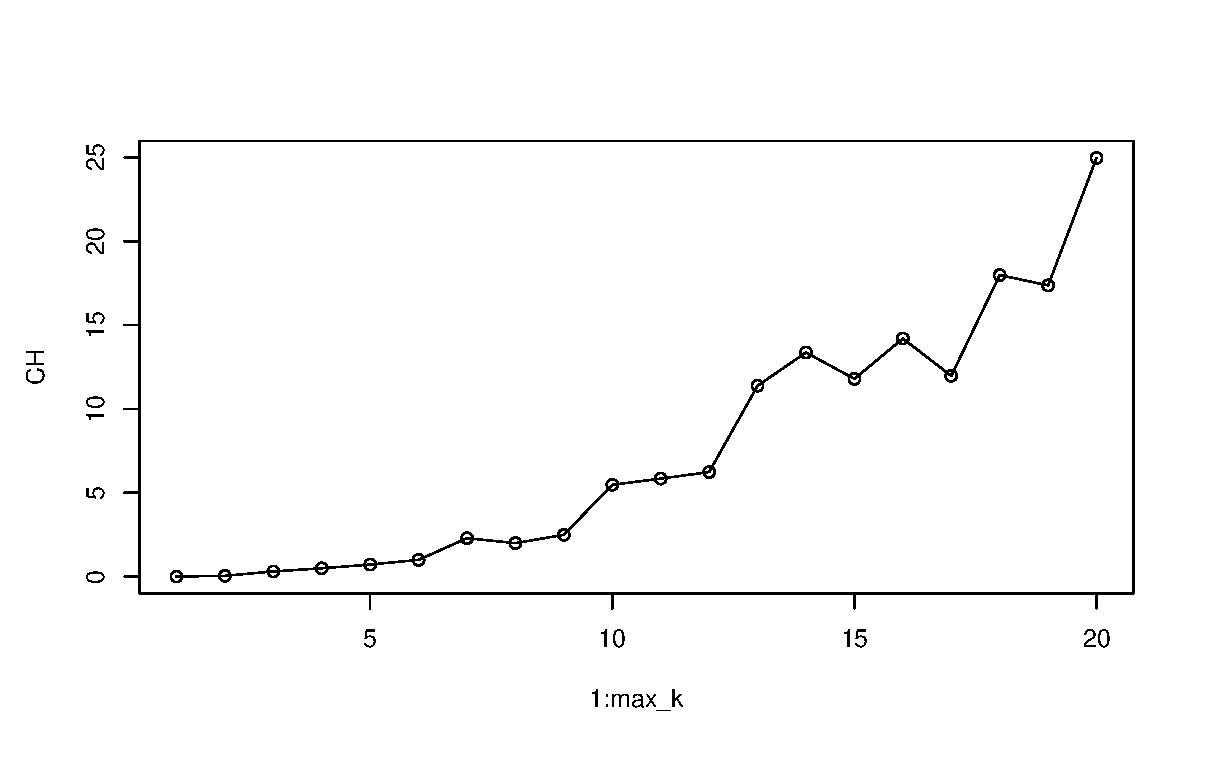
\includegraphics[width = 0.3\textwidth]{pics/hw2_data4_k_CH.eps}}\hfill
% \subfloat[H method]{ %
% 	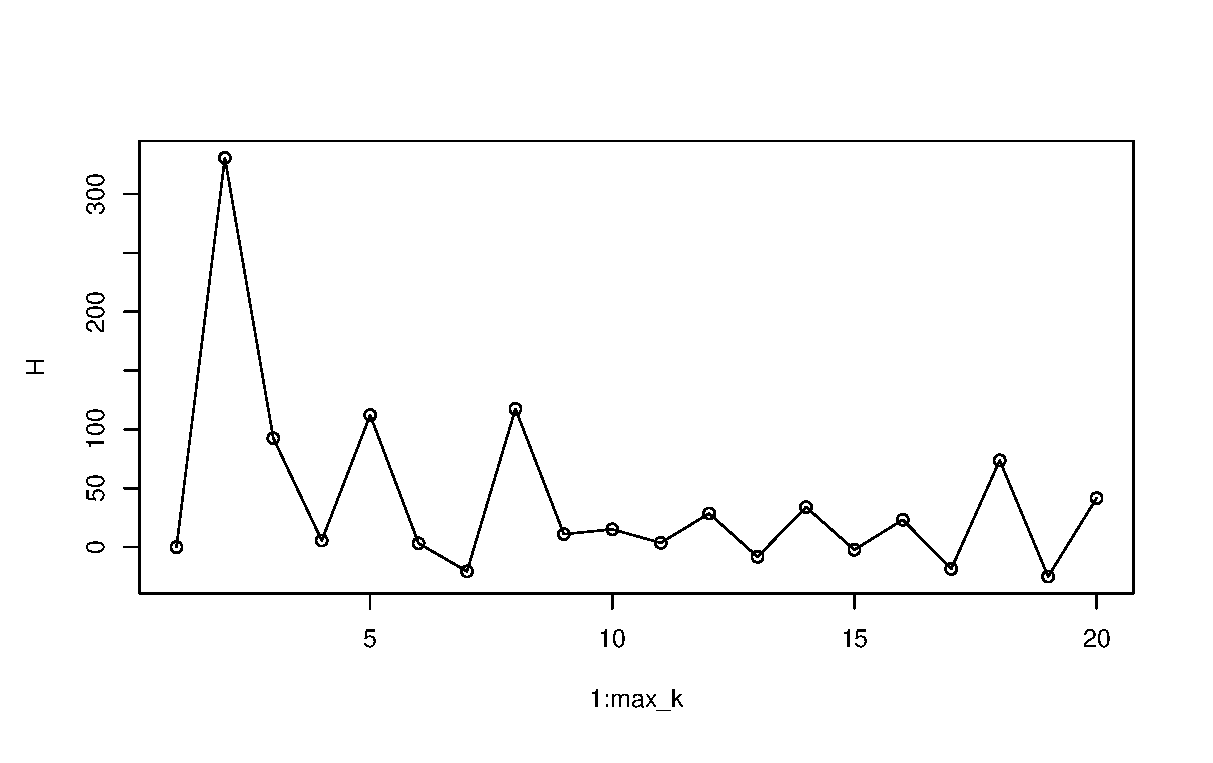
\includegraphics[width = 0.3\textwidth]{pics/hw2_data4_k_H.eps}}\hfill
% \subfloat[GAP statistic]{ %
% 	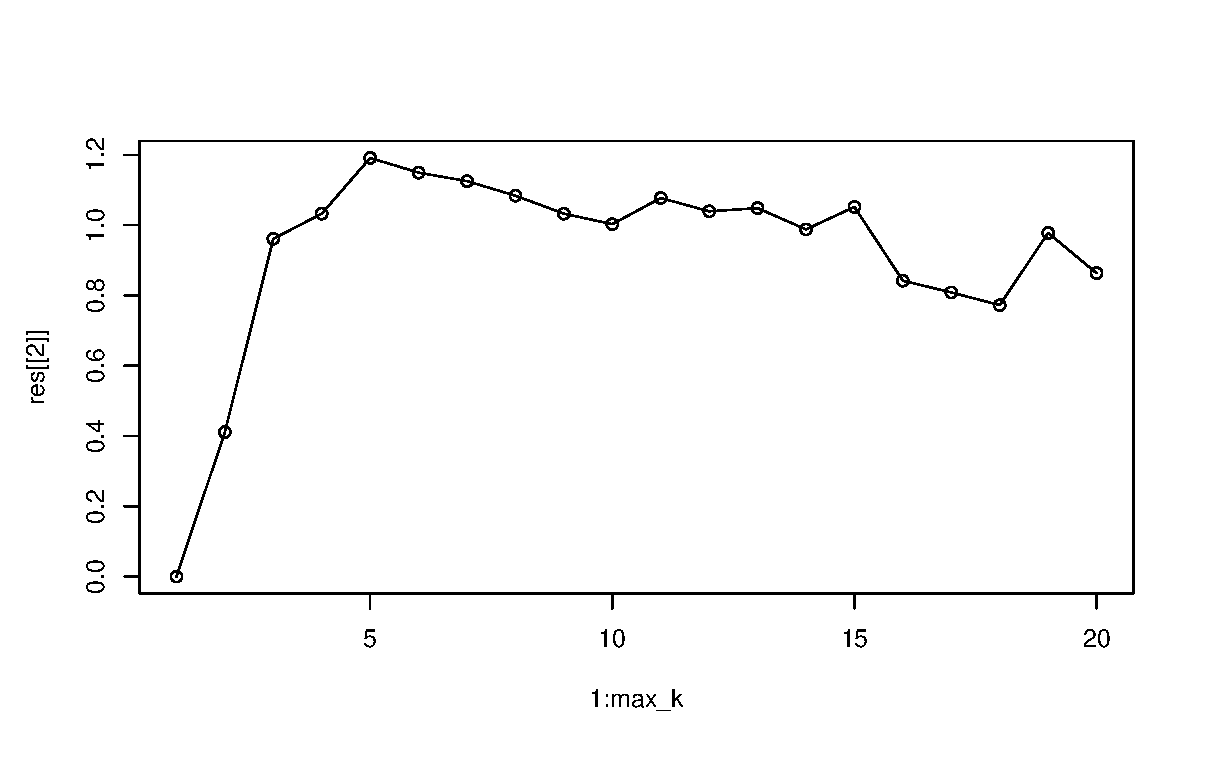
\includegraphics[width = 0.3\textwidth]{pics/hw2_data4_k_GAP.eps}}\hfill
% \caption{The three evaluating methods of choosing k for Data4.csv}
% \label{EVA Data2}
% \end{figure}
% }
% \solution{Analysis}{
% It is suprising that result of Calinski-Harabasz method does not agree with the other methods. I consider it as the result that I misunderstood the meaning of $W(k), B(k)$. I calculate the former as the target function of cluster; the latter as $\sum_{c_i, c_j \in C}\lVert c_i - c_j \rVert^2$, in which $C$ is the set of cluster centers.
% }

% \problem{3}{Use hierarchical clustering methods to cluster $Data_i.csv$}
% \solution{Solution}{
% The code of hierarchical clustering and the test script can be found from attachments(hierarchical\_clustering.R, hw1.3.R).
% }
% \solution{Result}{
% It is somehow embarrassing that I still did't know how to draw trees in R without $hcluster()$. The result can be shown is the attachments, (HC\_DATA1.txt and HC\_DATA2.txt). \\[3pt]
% Each result is a (n-1) * narg matrix, in which n is the number of data points and narg is the number of dims in each data point. Each row in the matrix(for example, A[1, ]) means a step when two points merged with each other; A[1, 1] and A[1, 2] merged into a new A[1, 1], and the point represented by A[1, 2] is abandoned. \\[3pt]
% It is possible to draw the tree and do Tree-Cut with the results.
% }

% \refgroup{
% \reference{a a a a  a a}
% \reference{b b b b b b}
% \reference{c c c c c c}
% \reference{b}

% }


\end{document}